

\chapter{Lists}

This chapter presents one of Python's most useful built-in types, lists.
You will also learn more about objects and what can happen when you have
more than one name for the same object.


\section{A list is a sequence}
\label{sequence}

Like a string, a {\bf list} is a sequence of values.  In a string, the
values are characters; in a list, they can be any type.  The values in
a list are called {\bf elements} or sometimes {\bf items}.
\index{list}
\index{type!list}
\index{element}
\index{sequence}
\index{item}

There are several ways to create a new list; the simplest is to
enclose the elements in square brackets (\verb"[" and \verb"]"):

\begin{verbatim}
[10, 20, 30, 40]
['crunchy frog', 'ram bladder', 'lark vomit']
\end{verbatim}
%
The first example is a list of four integers.  The second is a list of
three strings.  The elements of a list don't have to be the same type.
The following list contains a string, a float, an integer, and
(lo!) another list:

\begin{verbatim}
['spam', 2.0, 5, [10, 20]]
\end{verbatim}
%
A list within another list is {\bf nested}.
\index{nested list}
\index{list!nested}

A list that contains no elements is
called an empty list; you can create one with empty
brackets, \verb"[]".
\index{empty list}
\index{list!empty}

As you might expect, you can assign list values to variables:

\begin{verbatim}
>>> cheeses = ['Cheddar', 'Edam', 'Gouda']
>>> numbers = [42, 123]
>>> empty = []
>>> print(cheeses, numbers, empty)
['Cheddar', 'Edam', 'Gouda'] [42, 123] []
\end{verbatim}
%
\index{assignment}


\section{Lists are mutable}
\label{mutable}
\index{list!element}
\index{access}
\index{index}
\index{bracket operator}
\index{operator!bracket}

The syntax for accessing the elements of a list is the same as for
accessing the characters of a string---the bracket operator.  The
expression inside the brackets specifies the index.  Remember that the
indices start at 0:

\begin{verbatim}
>>> cheeses[0]
'Cheddar'
\end{verbatim}
%
Unlike strings, lists are mutable.  When the bracket operator appears
on the left side of an assignment, it identifies the element of the
list that will be assigned.
\index{mutability}

\begin{verbatim}
>>> numbers = [42, 123]
>>> numbers[1] = 5
>>> numbers
[42, 5]
\end{verbatim}
%
The one-eth element of {\tt numbers}, which
used to be 123, is now 5.
\index{index!starting at zero}
\index{zero, index starting at}

Figure~\ref{fig.liststate} shows
the state diagram for {\tt
cheeses}, {\tt numbers} and {\tt empty}:
\index{state diagram}
\index{diagram!state}

\begin{figure}
\centerline
{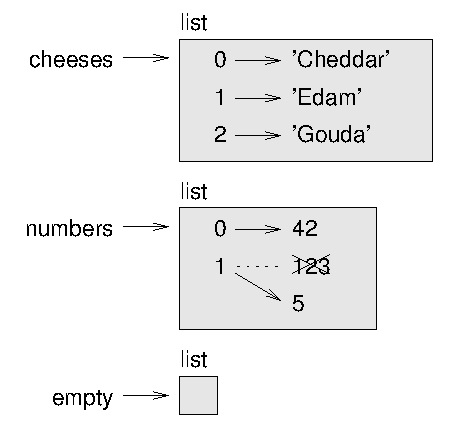
\includegraphics[scale=0.8]{../source/figs/liststate.pdf}}
\caption{State diagram.}
\label{fig.liststate}
\end{figure}

Lists are represented by boxes with the word ``list'' outside
and the elements of the list inside.  {\tt cheeses} refers to
a list with three elements indexed 0, 1 and 2.
{\tt numbers} contains two elements; the diagram shows that the
value of the second element has been reassigned from 123 to 5.
{\tt empty} refers to a list with no elements.
\index{item assignment}
\index{assignment!item}
\index{reassignment}

List indices work the same way as string indices:

\begin{itemize}

\item Any integer expression can be used as an index.

\item If you try to read or write an element that does not exist, you
get an {\tt IndexError}.
\index{exception!IndexError}
\index{IndexError}

\item If an index has a negative value, it counts backward from the
end of the list.

\end{itemize}
\index{list!index}

\index{list!membership}
\index{membership!list}
\index{in operator}
\index{operator!in}

The {\tt in} operator also works on lists.

\begin{verbatim}
>>> cheeses = ['Cheddar', 'Edam', 'Gouda']
>>> 'Edam' in cheeses
True
>>> 'Brie' in cheeses
False
\end{verbatim}


\section{Traversing a list}
\index{list!traversal}
\index{traversal!list}
\index{for loop}
\index{loop!for}
\index{statement!for}

The most common way to traverse the elements of a list is
with a {\tt for} loop.  The syntax is the same as for strings:

\begin{verbatim}
for cheese in cheeses:
    print(cheese)
\end{verbatim}
%
This works well if you only need to read the elements of the
list.  But if you want to write or update the elements, you
need the indices.  A common way to do that is to combine
the built-in functions {\tt range} and {\tt len}:
\index{looping!with indices}
\index{index!looping with}

\begin{verbatim}
for i in range(len(numbers)):
    numbers[i] = numbers[i] * 2
\end{verbatim}
%
This loop traverses the list and updates each element.  {\tt len}
returns the number of elements in the list.  {\tt range} returns
a list of indices from 0 to $n-1$, where $n$ is the length of
the list.  Each time through the loop {\tt i} gets the index
of the next element.  The assignment statement in the body uses
{\tt i} to read the old value of the element and to assign the
new value.
\index{item update}
\index{update!item}

A {\tt for} loop over an empty list never runs the body:

\begin{verbatim}
for x in []:
    print('This never happens.')
\end{verbatim}
%
Although a list can contain another list, the nested
list still counts as a single element.  The length of this list is
four:
\index{nested list}
\index{list!nested}

\begin{verbatim}
['spam', 1, ['Brie', 'Roquefort', 'Pol le Veq'], [1, 2, 3]]
\end{verbatim}



\section{List operations}
\index{list!operation}

The {\tt +} operator concatenates lists:
\index{concatenation!list}
\index{list!concatenation}

\begin{verbatim}
>>> a = [1, 2, 3]
>>> b = [4, 5, 6]
>>> c = a + b
>>> c
[1, 2, 3, 4, 5, 6]
\end{verbatim}
%
The {\tt *} operator repeats a list a given number of times:
\index{repetition!list}
\index{list!repetition}

\begin{verbatim}
>>> [0] * 4
[0, 0, 0, 0]
>>> [1, 2, 3] * 3
[1, 2, 3, 1, 2, 3, 1, 2, 3]
\end{verbatim}
%
The first example repeats {\tt [0]} four times.  The second example
repeats the list {\tt [1, 2, 3]} three times.


\section{List slices}
\index{slice operator}
\index{operator!slice}
\index{index!slice}
\index{list!slice}
\index{slice!list}

The slice operator also works on lists:

\begin{verbatim}
>>> t = ['a', 'b', 'c', 'd', 'e', 'f']
>>> t[1:3]
['b', 'c']
>>> t[:4]
['a', 'b', 'c', 'd']
>>> t[3:]
['d', 'e', 'f']
\end{verbatim}
%
If you omit the first index, the slice starts at the beginning.
If you omit the second, the slice goes to the end.  So if you
omit both, the slice is a copy of the whole list.
\index{list!copy}
\index{slice!copy}
\index{copy!slice}

\begin{verbatim}
>>> t[:]
['a', 'b', 'c', 'd', 'e', 'f']
\end{verbatim}
%
Since lists are mutable, it is often useful to make a copy
before performing operations that modify lists.
\index{mutability}

A slice operator on the left side of an assignment
can update multiple elements:
\index{slice!update}
\index{update!slice}

\begin{verbatim}
>>> t = ['a', 'b', 'c', 'd', 'e', 'f']
>>> t[1:3] = ['x', 'y']
>>> t
['a', 'x', 'y', 'd', 'e', 'f']
\end{verbatim}
%

% You can add elements to a list by squeezing them into an empty
% slice:

% % \begin{verbatim}
% >>> t = ['a', 'd', 'e', 'f']
% >>> t[1:1] = ['b', 'c']
% >>> print t
% ['a', 'b', 'c', 'd', 'e', 'f']
% \end{verbatim}
% \afterverb
%
% And you can remove elements from a list by assigning the empty list to
% them:

% % \begin{verbatim}
% >>> t = ['a', 'b', 'c', 'd', 'e', 'f']
% >>> t[1:3] = []
% >>> print t
% ['a', 'd', 'e', 'f']
% \end{verbatim}
% \afterverb
%
% But both of those operations can be expressed more clearly
% with list methods.


\section{List methods}
\index{list!method}
\index{method, list}

Python provides methods that operate on lists.  For example,
{\tt append} adds a new element to the end of a list:
\index{append method}
\index{method!append}

\begin{verbatim}
>>> t = ['a', 'b', 'c']
>>> t.append('d')
>>> t
['a', 'b', 'c', 'd']
\end{verbatim}
%
{\tt extend} takes a list as an argument and appends all of
the elements:
\index{extend method}
\index{method!extend}

\begin{verbatim}
>>> t1 = ['a', 'b', 'c']
>>> t2 = ['d', 'e']
>>> t1.extend(t2)
>>> t1
['a', 'b', 'c', 'd', 'e']
\end{verbatim}
%
This example leaves {\tt t2} unmodified.

{\tt sort} arranges the elements of the list from low to high:
\index{sort method}
\index{method!sort}

\begin{verbatim}
>>> t = ['d', 'c', 'e', 'b', 'a']
>>> t.sort()
>>> t
['a', 'b', 'c', 'd', 'e']
\end{verbatim}
%
Most list methods are void; they modify the list and return {\tt None}.
If you accidentally write {\tt t = t.sort()}, you will be disappointed
with the result.
\index{void method}
\index{method!void}
\index{None special value}
\index{special value!None}


\section{Map, filter and reduce}
\label{filter}

To add up all the numbers in a list, you can use a loop like this:

% see add.py

\begin{verbatim}
def add_all(t):
    total = 0
    for x in t:
        total += x
    return total
\end{verbatim}
%
{\tt total} is initialized to 0.  Each time through the loop,
{\tt x} gets one element from the list.  The {\tt +=} operator
provides a short way to update a variable.  This
{\bf augmented assignment statement},
\index{update operator}
\index{operator!update}
\index{assignment!augmented}
\index{augmented assignment}

\begin{verbatim}
    total += x
\end{verbatim}
%
is equivalent to

\begin{verbatim}
    total = total + x
\end{verbatim}
%
As the loop runs, {\tt total} accumulates the sum of the
elements; a variable used this way is sometimes called an
{\bf accumulator}.
\index{accumulator!sum}

Adding up the elements of a list is such a common operation
that Python provides it as a built-in function, {\tt sum}:

\begin{verbatim}
>>> t = [1, 2, 3]
>>> sum(t)
6
\end{verbatim}
%
An operation like this that combines a sequence of elements into
a single value is sometimes called {\bf reduce}.
\index{reduce pattern}
\index{pattern!reduce}
\index{traversal}

Sometimes you want to traverse one list while building
another.  For example, the following function takes a list of strings
and returns a new list that contains capitalized strings:

\begin{verbatim}
def capitalize_all(t):
    res = []
    for s in t:
        res.append(s.capitalize())
    return res
\end{verbatim}
%
{\tt res} is initialized with an empty list; each time through
the loop, we append the next element.  So {\tt res} is another
kind of accumulator.
\index{accumulator!list}

An operation like \verb"capitalize_all" is sometimes called a {\bf
map} because it ``maps'' a function (in this case the method {\tt
capitalize}) onto each of the elements in a sequence.
\index{map pattern}
\index{pattern!map}
\index{filter pattern}
\index{pattern!filter}

Another common operation is to select some of the elements from
a list and return a sublist.  For example, the following
function takes a list of strings and returns a list that contains
only the uppercase strings:

\begin{verbatim}
def only_upper(t):
    res = []
    for s in t:
        if s.isupper():
            res.append(s)
    return res
\end{verbatim}
%
{\tt isupper} is a string method that returns {\tt True} if
the string contains only upper case letters.

An operation like \verb"only_upper" is called a {\bf filter} because
it selects some of the elements and filters out the others.

Most common list operations can be expressed as a combination
of map, filter and reduce.


\section{Deleting elements}
\index{element deletion}
\index{deletion, element of list}

There are several ways to delete elements from a list.  If you
know the index of the element you want, you can use
{\tt pop}:
\index{pop method}
\index{method!pop}

\begin{verbatim}
>>> t = ['a', 'b', 'c']
>>> x = t.pop(1)
>>> t
['a', 'c']
>>> x
'b'
\end{verbatim}
%
{\tt pop} modifies the list and returns the element that was removed.
If you don't provide an index, it deletes and returns the
last element.

If you don't need the removed value, you can use the {\tt del}
operator:
\index{del operator}
\index{operator!del}

\begin{verbatim}
>>> t = ['a', 'b', 'c']
>>> del t[1]
>>> t
['a', 'c']
\end{verbatim}
%
If you know the element you want to remove (but not the index), you
can use {\tt remove}:
\index{remove method}
\index{method!remove}

\begin{verbatim}
>>> t = ['a', 'b', 'c']
>>> t.remove('b')
>>> t
['a', 'c']
\end{verbatim}
%
The return value from {\tt remove} is {\tt None}.
\index{None special value}
\index{special value!None}

To remove more than one element, you can use {\tt del} with
a slice index:

\begin{verbatim}
>>> t = ['a', 'b', 'c', 'd', 'e', 'f']
>>> del t[1:5]
>>> t
['a', 'f']
\end{verbatim}
%
As usual, the slice selects all the elements up to but not
including the second index.



\section{Lists and strings}
\index{list}
\index{string}
\index{sequence}

A string is a sequence of characters and a list is a sequence
of values, but a list of characters is not the same as a
string.  To convert from a string to a list of characters,
you can use {\tt list}:
\index{list!function}
\index{function!list}

\begin{verbatim}
>>> s = 'spam'
>>> t = list(s)
>>> t
['s', 'p', 'a', 'm']
\end{verbatim}
%
Because {\tt list} is the name of a built-in function, you should
avoid using it as a variable name.  I also avoid {\tt l} because
it looks too much like {\tt 1}.  So that's why I use {\tt t}.

The {\tt list} function breaks a string into individual letters.  If
you want to break a string into words, you can use the {\tt split}
method:
\index{split method}
\index{method!split}

\begin{verbatim}
>>> s = 'pining for the fjords'
>>> t = s.split()
>>> t
['pining', 'for', 'the', 'fjords']
\end{verbatim}
%
An optional argument called a {\bf delimiter} specifies which
characters to use as word boundaries.
The following example
uses a hyphen as a delimiter:
\index{optional argument}
\index{argument!optional}
\index{delimiter}

\begin{verbatim}
>>> s = 'spam-spam-spam'
>>> delimiter = '-'
>>> t = s.split(delimiter)
>>> t
['spam', 'spam', 'spam']
\end{verbatim}
%
{\tt join} is the inverse of {\tt split}.  It
takes a list of strings and
concatenates the elements.  {\tt join} is a string method,
so you have to invoke it on the delimiter and pass the
list as a parameter:
\index{join method}
\index{method!join}
\index{concatenation}

\begin{verbatim}
>>> t = ['pining', 'for', 'the', 'fjords']
>>> delimiter = ' '
>>> s = delimiter.join(t)
>>> s
'pining for the fjords'
\end{verbatim}
%
In this case the delimiter is a space character, so
{\tt join} puts a space between words.  To concatenate
strings without spaces, you can use the empty string,
\verb"''", as a delimiter.
\index{empty string}
\index{string!empty}


\section{Objects and values}
\label{equivalence}
\index{object}
\index{value}

If we run these assignment statements:

\begin{verbatim}
a = 'banana'
b = 'banana'
\end{verbatim}
%
We know that {\tt a} and {\tt b} both refer to a
string, but we don't
know whether they refer to the {\em same} string.
There are two possible states, shown in Figure~\ref{fig.list1}.
\index{aliasing}

\begin{figure}
\centerline
{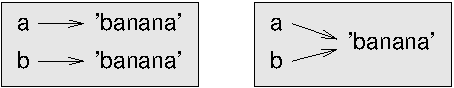
\includegraphics[scale=0.8]{../source/figs/list1.pdf}}
\caption{State diagram.}
\label{fig.list1}
\end{figure}

In one case, {\tt a} and {\tt b} refer to two different objects that
have the same value.  In the second case, they refer to the same
object.
\index{is operator}
\index{operator!is}

To check whether two variables refer to the same object, you can
use the {\tt is} operator.

\begin{verbatim}
>>> a = 'banana'
>>> b = 'banana'
>>> a is b
True
\end{verbatim}
%
In this example, Python only created one string object, and both {\tt
  a} and {\tt b} refer to it.  But when you create two lists, you get
two objects:

\begin{verbatim}
>>> a = [1, 2, 3]
>>> b = [1, 2, 3]
>>> a is b
False
\end{verbatim}
%
So the state diagram looks like Figure~\ref{fig.list2}.
\index{state diagram}
\index{diagram!state}

\begin{figure}
\centerline
{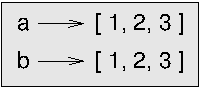
\includegraphics[scale=0.8]{../source/figs/list2.pdf}}
\caption{State diagram.}
\label{fig.list2}
\end{figure}

In this case we would say that the two lists are {\bf equivalent},
because they have the same elements, but not {\bf identical}, because
they are not the same object.  If two objects are identical, they are
also equivalent, but if they are equivalent, they are not necessarily
identical.
\index{equivalence}
\index{identity}

Until now, we have been using ``object'' and ``value''
interchangeably, but it is more precise to say that an object has a
value.  If you evaluate {\tt [1, 2, 3]}, you get a list
object whose value is a sequence of integers.  If another
list has the same elements, we say it has the same value, but
it is not the same object.
\index{object}
\index{value}


\section{Aliasing}
\index{aliasing}
\index{reference!aliasing}

If {\tt a} refers to an object and you assign {\tt b = a},
then both variables refer to the same object:

\begin{verbatim}
>>> a = [1, 2, 3]
>>> b = a
>>> b is a
True
\end{verbatim}
%
The state diagram looks like Figure~\ref{fig.list3}.
\index{state diagram}
\index{diagram!state}

\begin{figure}
\centerline
{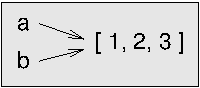
\includegraphics[scale=0.8]{../source/figs/list3.pdf}}
\caption{State diagram.}
\label{fig.list3}
\end{figure}

The association of a variable with an object is called a {\bf
reference}.  In this example, there are two references to the same
object.
\index{reference}

An object with more than one reference has more
than one name, so we say that the object is {\bf aliased}.
\index{mutability}

If the aliased object is mutable, changes made with one alias affect
the other:

\begin{verbatim}
>>> b[0] = 42
>>> a
[42, 2, 3]
\end{verbatim}
%
Although this behavior can be useful, it is error-prone.  In general,
it is safer to avoid aliasing when you are working with mutable
objects.
\index{immutability}

For immutable objects like strings, aliasing is not as much of a
problem.  In this example:

\begin{verbatim}
a = 'banana'
b = 'banana'
\end{verbatim}
%
It almost never makes a difference whether {\tt a} and {\tt b} refer
to the same string or not.


\section{List arguments}
\label{list.arguments}
\index{list!as argument}
\index{argument}
\index{argument!list}
\index{reference}
\index{parameter}

When you pass a list to a function, the function gets a reference to
the list.  If the function modifies the list, the caller sees
the change.  For example, \verb"delete_head" removes the first element
from a list:

\begin{verbatim}
def delete_head(t):
    del t[0]
\end{verbatim}
%
Here's how it is used:

\begin{verbatim}
>>> letters = ['a', 'b', 'c']
>>> delete_head(letters)
>>> letters
['b', 'c']
\end{verbatim}
%
The parameter {\tt t} and the variable {\tt letters} are
aliases for the same object.  The stack diagram looks like
Figure~\ref{fig.stack5}.
\index{stack diagram}
\index{diagram!stack}

\begin{figure}
\centerline
{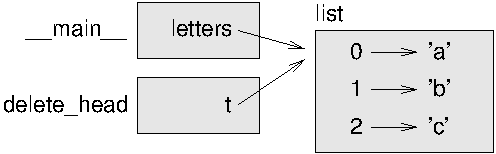
\includegraphics[scale=0.8]{../source/figs/stack5.pdf}}
\caption{Stack diagram.}
\label{fig.stack5}
\end{figure}

Since the list is shared by two frames, I drew
it between them.

It is important to distinguish between operations that
modify lists and operations that create new lists.  For
example, the {\tt append} method modifies a list, but the
{\tt +} operator creates a new list:
\index{append method}
\index{method!append}
\index{list!concatenation}
\index{concatenation!list}
%
\begin{verbatim}
>>> t1 = [1, 2]
>>> t2 = t1.append(3)
>>> t1
[1, 2, 3]
>>> t2
None
\end{verbatim}
%
{\tt append} modifies the list and returns {\tt None}.
%
\begin{verbatim}
>>> t3 = t1 + [4]
>>> t1
[1, 2, 3]
>>> t3
[1, 2, 3, 4]
>>> t1
\end{verbatim}
%
The {\tt +} operator creates a new list and leaves the
original list unchanged.

This difference is important when you write functions that
are supposed to modify lists.  For example, this function
{\em does not} delete the head of a list:
%
\begin{verbatim}
def bad_delete_head(t):
    t = t[1:]              # WRONG!
\end{verbatim}
%
The slice operator creates a new list and the assignment
makes {\tt t} refer to it, but that doesn't affect the caller.
\index{slice operator}
\index{operator!slice}
%
\begin{verbatim}
>>> t4 = [1, 2, 3]
>>> bad_delete_head(t4)
>>> t4
[1, 2, 3]
\end{verbatim}
%
At the beginning of \verb"bad_delete_head", {\tt t} and {\tt t4}
refer to the same list.  At the end, {\tt t} refers to a new list,
but {\tt t4} still refers to the original, unmodified list.

An alternative is to write a function that creates and
returns a new list.  For
example, {\tt tail} returns all but the first
element of a list:

\begin{verbatim}
def tail(t):
    return t[1:]
\end{verbatim}
%
This function leaves the original list unmodified.
Here's how it is used:

\begin{verbatim}
>>> letters = ['a', 'b', 'c']
>>> rest = tail(letters)
>>> rest
['b', 'c']
\end{verbatim}



\section{Debugging}
\index{debugging}

Careless use of lists (and other mutable objects)
can lead to long hours of debugging.  Here are some common
pitfalls and ways to avoid them:

\begin{enumerate}

\item Most list methods modify the argument and
  return {\tt None}.  This is the opposite of the string methods,
  which return a new string and leave the original alone.

If you are used to writing string code like this:

\begin{verbatim}
word = word.strip()
\end{verbatim}

It is tempting to write list code like this:

\begin{verbatim}
t = t.sort()           # WRONG!
\end{verbatim}
\index{sort method}
\index{method!sort}

Because {\tt sort} returns {\tt None}, the
next operation you perform with {\tt t} is likely to fail.

Before using list methods and operators, you should read the
documentation carefully and then test them in interactive mode.

\item Pick an idiom and stick with it.

Part of the problem with lists is that there are too many
ways to do things.  For example, to remove an element from
a list, you can use {\tt pop}, {\tt remove}, {\tt del},
or even a slice assignment.

To add an element, you can use the {\tt append} method or
the {\tt +} operator.  Assuming that {\tt t} is a list and
{\tt x} is a list element, these are correct:

\begin{verbatim}
t.append(x)
t = t + [x]
t += [x]
\end{verbatim}

And these are wrong:

\begin{verbatim}
t.append([x])          # WRONG!
t = t.append(x)        # WRONG!
t + [x]                # WRONG!
t = t + x              # WRONG!
\end{verbatim}

Try out each of these examples in interactive mode to make sure
you understand what they do.  Notice that only the last
one causes a runtime error; the other three are legal, but they
do the wrong thing.


\item Make copies to avoid aliasing.
\index{aliasing!copying to avoid}
\index{copy!to avoid aliasing}

If you want to use a method like {\tt sort} that modifies
the argument, but you need to keep the original list as
well, you can make a copy.

\begin{verbatim}
>>> t = [3, 1, 2]
>>> t2 = t[:]
>>> t2.sort()
>>> t
[3, 1, 2]
>>> t2
[1, 2, 3]
\end{verbatim}

In this example you could also use the built-in function {\tt sorted},
which returns a new, sorted list and leaves the original alone.

\begin{verbatim}
>>> t2 = sorted(t)
>>> t
[3, 1, 2]
>>> t2
[1, 2, 3]
\end{verbatim}

\end{enumerate}



\section{Glossary}

\begin{description}

\item[list:] A sequence of values.
\index{list}

\item[element:] One of the values in a list (or other sequence),
also called items.
\index{element}

\item[nested list:] A list that is an element of another list.
\index{nested list}

\item[accumulator:] A variable used in a loop to add up or
accumulate a result.
\index{accumulator}

\item[augmented assignment:] A statement that updates the value
of a variable using an operator like \verb"+=".
\index{assignment!augmented}
\index{augmented assignment}
\index{traversal}

\item[reduce:] A processing pattern that traverses a sequence
and accumulates the elements into a single result.
\index{reduce pattern}
\index{pattern!reduce}

\item[map:] A processing pattern that traverses a sequence and
performs an operation on each element.
\index{map pattern}
\index{pattern!map}

\item[filter:] A processing pattern that traverses a list and
selects the elements that satisfy some criterion.
\index{filter pattern}
\index{pattern!filter}

\item[object:] Something a variable can refer to.  An object
has a type and a value.
\index{object}

\item[equivalent:] Having the same value.
\index{equivalent}

\item[identical:] Being the same object (which implies equivalence).
\index{identical}

\item[reference:] The association between a variable and its value.
\index{reference}

\item[aliasing:] A circumstance where two or more variables refer to the same
object.
\index{aliasing}

\item[delimiter:] A character or string used to indicate where a
string should be split.
\index{delimiter}

\end{description}


\section{Exercises}

You can download solutions to these exercises from
\url{http://thinkpython2.com/code/list_exercises.py}.

\begin{exercise}

Write a function called \verb"nested_sum" that takes a list of lists
of integers and adds up the elements from all of the nested lists.
For example:

\begin{verbatim}
>>> t = [[1, 2], [3], [4, 5, 6]]
>>> nested_sum(t)
21
\end{verbatim}

\end{exercise}

\begin{exercise}
\label{cumulative}
\index{cumulative sum}

Write a function called {\tt cumsum} that takes a list of numbers and
returns the cumulative sum; that is, a new list where the $i$th
element is the sum of the first $i+1$ elements from the original list.
For example:

\begin{verbatim}
>>> t = [1, 2, 3]
>>> cumsum(t)
[1, 3, 6]
\end{verbatim}

\end{exercise}

\begin{exercise}

Write a function called \verb"middle" that takes a list and
returns a new list that contains all but the first and last
elements.  For example:

\begin{verbatim}
>>> t = [1, 2, 3, 4]
>>> middle(t)
[2, 3]
\end{verbatim}

\end{exercise}

\begin{exercise}

Write a function called \verb"chop" that takes a list, modifies it
by removing the first and last elements, and returns {\tt None}.
For example:

\begin{verbatim}
>>> t = [1, 2, 3, 4]
>>> chop(t)
>>> t
[2, 3]
\end{verbatim}

\end{exercise}


\begin{exercise}
Write a function called \verb"is_sorted" that takes a list as a
parameter and returns {\tt True} if the list is sorted in ascending
order and {\tt False} otherwise.  For example:

\begin{verbatim}
>>> is_sorted([1, 2, 2])
True
>>> is_sorted(['b', 'a'])
False
\end{verbatim}

\end{exercise}


\begin{exercise}
\label{anagram}
\index{anagram}

Two words are anagrams if you can rearrange the letters from one
to spell the other.  Write a function called \verb"is_anagram"
that takes two strings and returns {\tt True} if they are anagrams.
\end{exercise}



\begin{exercise}
\label{duplicate}
\index{duplicate}
\index{uniqueness}

Write a function called \verb"has_duplicates" that takes
a list and returns {\tt True} if there is any element that
appears more than once.  It should not modify the original
list.

\end{exercise}


\begin{exercise}

This exercise pertains to the so-called Birthday Paradox, which you
can read about at \url{http://en.wikipedia.org/wiki/Birthday_paradox}.
\index{birthday paradox}

If there are 23 students in your class, what are the chances
that two of you have the same birthday?  You can estimate this
probability by generating random samples of 23 birthdays
and checking for matches.  Hint: you can generate random birthdays
with the {\tt randint} function in the {\tt random} module.
\index{random module}
\index{module!random}
\index{randint function}
\index{function!randint}

You can download my
solution from \url{http://thinkpython2.com/code/birthday.py}.

\end{exercise}



\begin{exercise}
\index{append method}
\index{method append}
\index{list!concatenation}
\index{concatenation!list}

Write a function that reads the file {\tt words.txt} and builds
a list with one element per word.  Write two versions of
this function, one using the {\tt append} method and the
other using the idiom {\tt t = t + [x]}.  Which one takes
longer to run?  Why?

Solution: \url{http://thinkpython2.com/code/wordlist.py}.
\index{time module}
\index{module!time}

\end{exercise}


\begin{exercise}
\label{wordlist1}
\label{bisection}
\index{membership!bisection search}
\index{bisection search}
\index{search, bisection}
\index{membership!binary search}
\index{binary search}
\index{search, binary}

To check whether a word is in the word list, you could use
the {\tt in} operator, but it would be slow because it searches
through the words in order.

Because the words are in alphabetical order, we can speed things up
with a bisection search (also known as binary search), which is
similar to what you do when you look a word up in the dictionary.  You
start in the middle and check to see whether the word you are looking
for comes before the word in the middle of the list.  If so, you
search the first half of the list the same way.  Otherwise you search
the second half.

Either way, you cut the remaining search space in half.  If the
word list has 113,809 words, it will take about 17 steps to
find the word or conclude that it's not there.

Write a function called \verb"in_bisect" that takes a sorted list
and a target value and returns the index of the value
in the list if it's there, or {\tt None} if it's not.
\index{bisect module}
\index{module!bisect}

Or you could read the documentation of the {\tt bisect} module
and use that!  Solution: \url{http://thinkpython2.com/code/inlist.py}.

\end{exercise}

\begin{exercise}
\index{reverse word pair}

Two words are a ``reverse pair'' if each is the reverse of the
other.  Write a program that finds all the reverse pairs in the
word list.  Solution: \url{http://thinkpython2.com/code/reverse_pair.py}.

\end{exercise}

\begin{exercise}
\index{interlocking words}

Two words ``interlock'' if taking alternating letters from each forms
a new word.  For example, ``shoe'' and ``cold''
interlock to form ``schooled''.
Solution: \url{http://thinkpython2.com/code/interlock.py}.
Credit: This exercise is inspired by an example at \url{http://puzzlers.org}.

\begin{enumerate}

\item Write a program that finds all pairs of words that interlock.
  Hint: don't enumerate all pairs!

\item Can you find any words that are three-way interlocked; that is,
  every third letter forms a word, starting from the first, second or
  third?

\end{enumerate}
\end{exercise}

